\subsection{Schraubenauslegung \hfill ME}
\begin{footnotesize}
    \begin{minipage}{0.49\linewidth}
        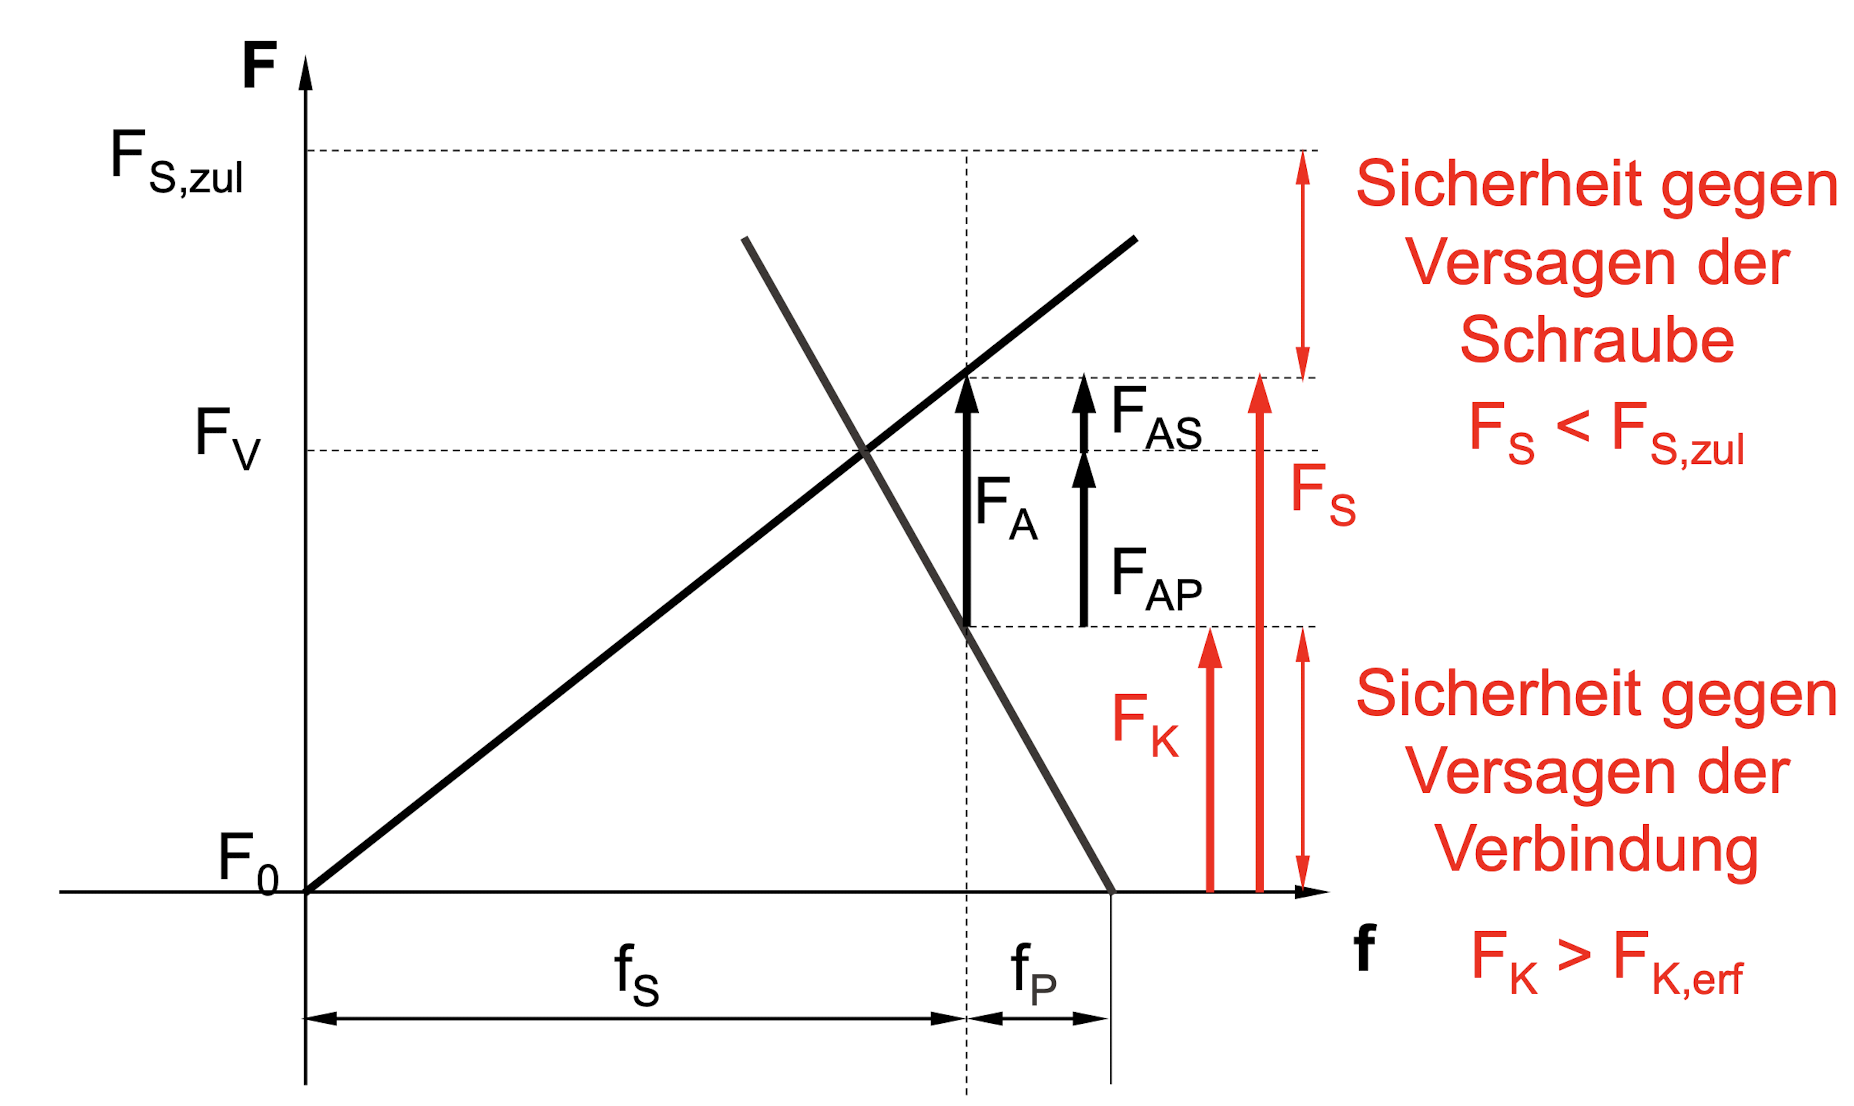
\includegraphics[width = 1.0\linewidth]{src/images/MAEIP_Schraubenauslegung1}
    \end{minipage}
    \begin{minipage}{0.49\linewidth}
        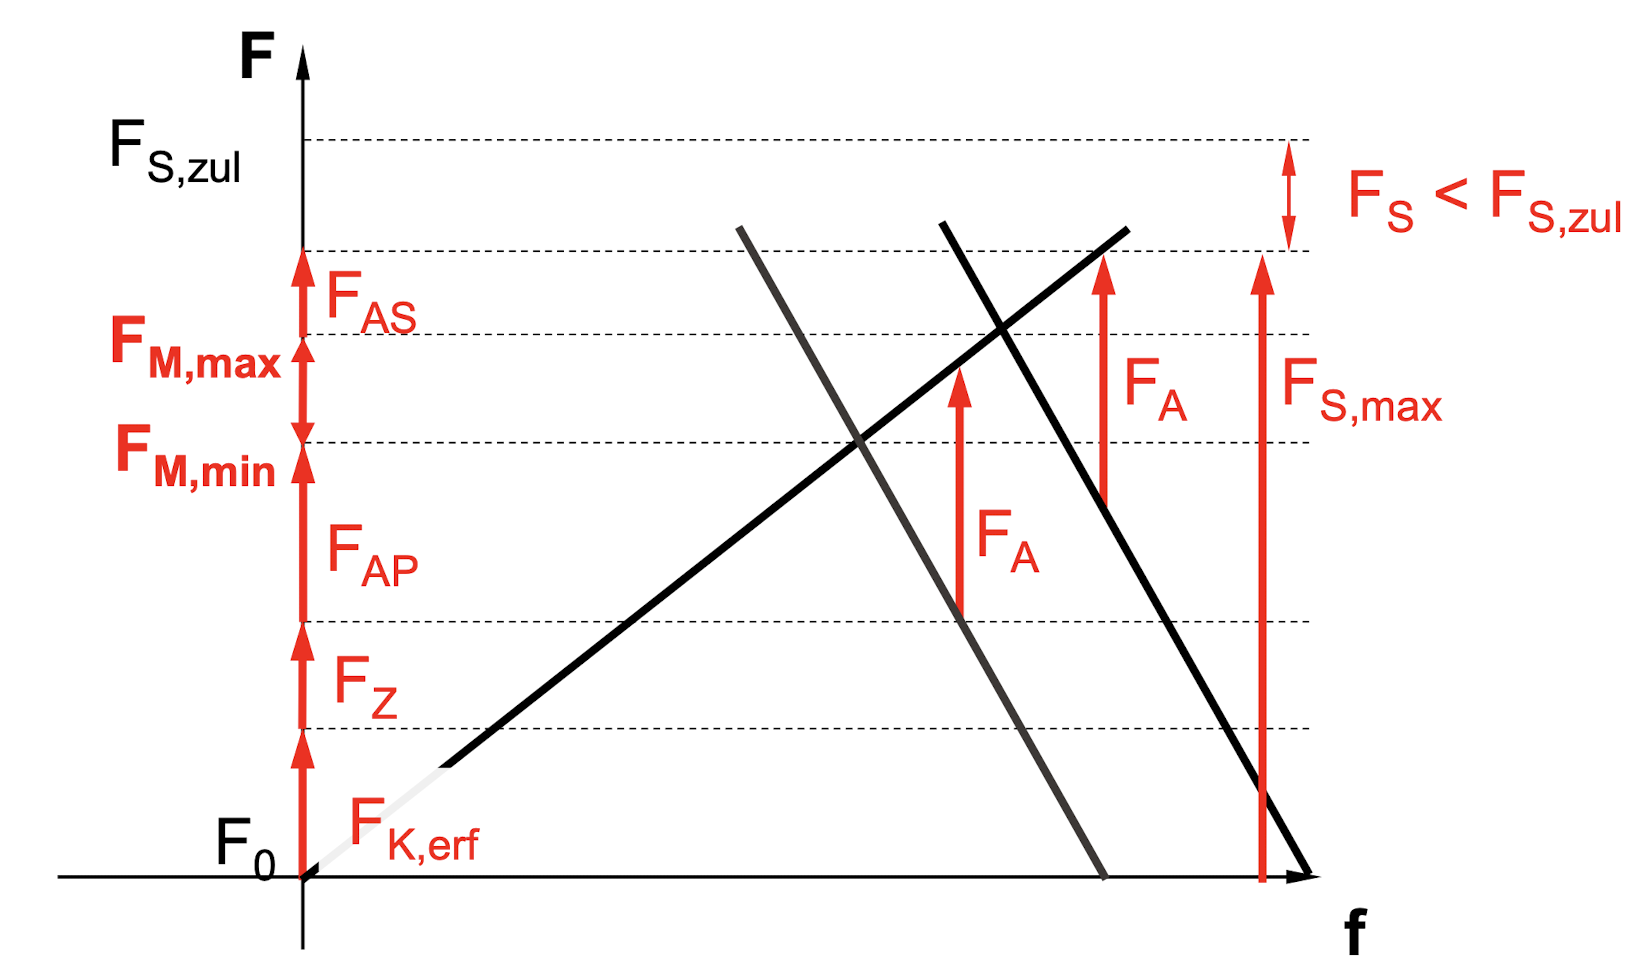
\includegraphics[width = 1.0\linewidth]{src/images/MAEIP_Schraubenauslegung2}
    \end{minipage}
    \begin{empheq}[box=\fbox]{align*}
        \scriptstyle F_{V, \text{min}} = F_{Kl, \text{erf}} + F_{BT} + F_Z \quad \mid \quad \sigma_V = \sqrt{\sigma_z^2 + 3 \cdot \tau_t^2}
        \\F_{V, \text{max}} = k_A \cdot F_{V, \text{min}} \quad \mid \quad F_{S, \text{max}} = F_{V, \text{max}} + F_{BS}
        \\ \scriptstyle F_{BS} = \frac{\delta_T}{\delta_S + \delta_T} F_B \quad \mid \quad F_{BT} = \frac{\delta_S}{\delta_S + \delta_T} F_B
        \\ \Delta f = F_BS \delta_S = F_{BT} \delta_T \quad \mid \quad F_Z = \frac{f_Z}{\delta_S + \delta_T}
    \end{empheq}
    \begin{scriptsize}
        \begin{minipage}{0.53\linewidth}
            \begin{empheq}[box=\fbox]{align*}
                F_{V, \text{min}} &= \text{Min. Anziehkraft}
                \\F_{BT}, F_{BS} &= \text{Axiale Betriebslast}
                \\&\text{ auf Platten / Schrauben}
                \\F_{V, \text{max}} &= \text{Max. Anziehkraft}
                \\\sigma_z &= \text{Max. Zugspannung}
                \\R_e &= \text{Streckgrenze}
            \end{empheq}
        \end{minipage}
        \begin{minipage}{0.45\linewidth}
            \begin{empheq}[box=\fbox]{align*}
                F_{Kl, \text{erf}} &= \text{erf. Klemmkraft}
                \\F_Z &= \text{Setzkraftverlust}
                \\k_A &= \text{Anziehfaktor}
                \\\tau_t &= \text{Max. Schubspannung}
                \\\sigma_V &= \text{Max. Vergleichsp.}
            \end{empheq}
        \end{minipage}
    \end{scriptsize}    
\end{footnotesize}